% Website adaptation of the visual setup in:
%   Chandler Squires, Anna Seigal, Salil Bhate, Caroline Uhler,
%   "Linear Causal Disentanglement via Interventions", ICML 2023, Fig. 1.
%   arXiv:2211.16467.
%
% The arXiv source includes that figure as an externally generated PDF
% (content/figures/pictures/latent-causal-model.pdf), not TikZ; this file is an
% original TikZ redraw of it. Change from the paper: the single observation map
% X = GZ is split into two observed groups X = G_X Z and Y = G_Y Z fed by the
% same latent DAG, as in the multimodal setting of the website project.
% See the publication for the original figure's rights.

\documentclass[tikz,border=4pt]{standalone}
\usepackage{amsmath}
\usetikzlibrary{arrows.meta}

\definecolor{paper}{HTML}{F7F5F0}
\definecolor{ink}{HTML}{18202A}
\definecolor{muted}{HTML}{65707A}
\definecolor{line}{HTML}{D9D6CE}
\definecolor{accent}{HTML}{1C5A76}
\definecolor{accentdark}{HTML}{123D51}
\definecolor{coral}{HTML}{D2604A}

\begin{document}
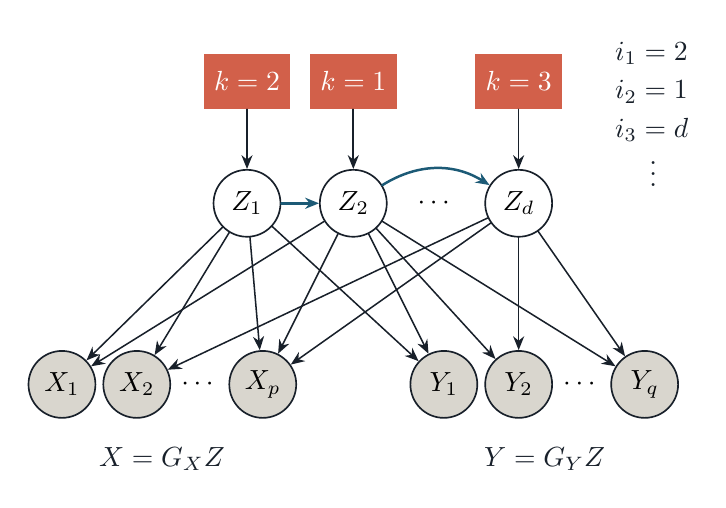
\begin{tikzpicture}[
  >={Stealth[length=5pt,width=4pt]},
  every path/.style={line cap=round},
  latent/.style={circle, draw=ink, line width=.6pt, fill=white, minimum size=8.5mm, inner sep=0pt},
  observed/.style={circle, draw=ink, line width=.6pt, fill=line, minimum size=8.5mm, inner sep=0pt},
  context/.style={rectangle, fill=coral, text=white, minimum width=11mm, minimum height=7mm, inner sep=1pt},
  mix/.style={->, ink, line width=.55pt},
  dag/.style={->, accent, line width=.9pt},
]

% ---------- latent causal model ----------
\node[latent] (z1) at (-1.35,0) {$Z_1$};
\node[latent] (z2) at (0,0)     {$Z_2$};
\node         at (1.05,0)       {$\cdots$};
\node[latent] (zd) at (2.1,0)   {$Z_d$};

\draw[dag] (z1) -- (z2);
\draw[dag] (z2) to[bend left=32] (zd);

% ---------- interventional contexts (one perfect intervention per latent) ----------
\node[context] (k2) at (-1.35,1.55) {$k=2$};
\node[context] (k1) at (0,1.55)     {$k=1$};
\node[context] (k3) at (2.1,1.55)   {$k=3$};
\foreach \k/\z in {k2/z1, k1/z2, k3/zd}
  \draw[->, ink, line width=.6pt] (\k) -- (\z);

\node[anchor=west, ink] at (3.2,1.1) {$
  \begin{aligned}
    i_1 &= 2\\[-1pt] i_2 &= 1\\[-1pt] i_3 &= d\\[-5pt] &\;\,\vdots
  \end{aligned}$};

% ---------- two observed groups ----------
\node[observed] (x1) at (-3.7,-2.3) {$X_1$};
\node[observed] (x2) at (-2.75,-2.3) {$X_2$};
\node           at (-1.95,-2.3)      {$\cdots$};
\node[observed] (xp) at (-1.15,-2.3) {$X_p$};

\node[observed] (y1) at (1.15,-2.3) {$Y_1$};
\node[observed] (y2) at (2.1,-2.3)  {$Y_2$};
\node           at (2.9,-2.3)       {$\cdots$};
\node[observed] (yq) at (3.7,-2.3)  {$Y_q$};

\foreach \z/\x in {z1/x1, z1/x2, z1/xp, z1/y1,
                   z2/x1, z2/xp, z2/y1, z2/y2, z2/yq,
                   zd/x2, zd/xp, zd/y2, zd/yq}
  \draw[mix] (\z) -- (\x);

\node[ink] at (-2.43,-3.25) {$X = G_X Z$};
\node[ink] at (2.43,-3.25)  {$Y = G_Y Z$};

\end{tikzpicture}
\end{document}
